%!TEX root = ../sbc-template.tex
A solução proposta para a realização deste trabalho compreende a caracterização da tarefa de aprendizado, exposta na Seção \ref{subsec:tarefa}. A descrição do conjunto de dados estão na Seção \ref{subsec:dataset}. A Seção \ref{subsec:limpeza} compreende a limpeza, o pré-processamento e a consolidação do conjunto de dados. Por fim, na Seção \ref{subsec:modelos} estão os modelos e hiperparâmetros de CNNs considerados.
\subsection{Tarefa de Aprendizado}\label{subsec:tarefa}
A tarefa de aprendizado considerada para a estimação de idade de telespectadores é a regresssão. Neste contexto, uma imagem em cores RGB de dimensões $224 \times 224$ pixels contendo uma face humana centralizada será fornecida como entrada. A saída desejada é a estimativa de idade, em anos, da pessoa correspondente, conforme exemplificado na Figura \ref{fig:deniro_cnn}. Esta tarefa será abordada segundo o paradigma de aprendizado supervisionado.

\begin{figure}[h!]
  \centering
     \caption{Tarefa de aprendizado}
     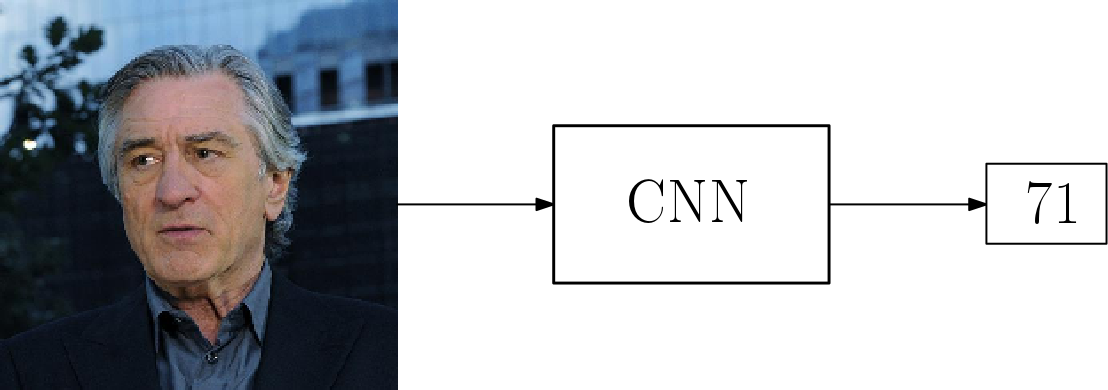
\includegraphics[width=0.8\textwidth]{img/deniro_cnn}
     \label{fig:deniro_cnn}
\end{figure}

Os dados disponíveis para este contexto serão particionados em três conjuntos disjuntos, sendo $70\%$ reservados para o treino, $10\%$ para validação e $20\%$ para teste. Esta partição obedece à tecnica \emph{Holdout} de validação cruzada \cite{brink2016real}.

Os modelos propostos para esta tarefa terão seu desempenho aferido perante os dados do conjunto de testes de acordo com a métrica de desempenho \emph{Root Mean Squared Error} (RMSE). Esta métrica considera a diferença entre cada um dos valores previstos $\hat{y}$ e os reais $y$, e posteriormente quantifica uma média imune à variação positiva ou negativa desta diferença. A Equação \ref{eq:rmse} denota o cálculo do RMSE \cite{brink2016real}.

\begin{equation}\label{eq:rmse}
     \textrm{RMSE} = \sqrt{\frac{1}{n} \sum_{i=1}^n (y_i - \hat{y})^2}.
\end{equation}

\subsection{Conjunto de Dados}\label{subsec:dataset}
%!TEX root = ../sbc-template.tex
Para a tarefa de aprendizado apresentada, dispôs-se da base de dados experimentais IMDb, composta de $452.132$ exemplares contendo imagens e outras informações de $20.284$ dos atores mais populares listados no site IMDb. O conjunto de dados foi construído utilizando técnicas de \emph{web crawling} aplicadas aos perfis de atores do site, em que foram coletadas todas as imagens relacionadas à celebridade, além de informações como data de nascimento, nome e gênero \cite{IMDb_derivada}.

A base de imagens oriunda do site IMDb foi organizada por Rothe et al. considerando uma tarefa de aprendizado análoga à deste trabalho, conforme mencionado na Seção  \ref{sec:trab_relac} \cite{rothe2015dex}.  Nesta base, há também as coordenadas da localização de um rosto detectado na imagem, além de uma pontuação atribuída ao rosto produzida pelo detector de face, quantificando o grau de certeza na detecção do rosto. Partindo da possibilidade de haver mais de um rosto por imagem, uma segunda pontuação é atribuída pelo detector, referente ao grau de certeza de que há outro rosto na mesma imagem.

Neste contexto, cada exemplo deste conjunto de dados é referente a uma imagem, cujos meta-dados estão descritos em seus atributos, que compreendem o nome, gênero, data de nascimento e um número de identificação da celebridade cujo perfil estava atrelado à imagem, o endereço da foto em disco, a suposta localização da face da celebridade, e pontuações referentes a duas possíveis faces encontradas. Assim, há exemplos de imagens em que há apenas um rosto, como mostrado na Figura \ref{tab:um_deniro}. Já na Figura \ref{tab:dois_deniro_correto} está o exemplo de uma imagem onde há mais de um rosto, porém a localização do rosto está correta. Por fim, na Figura \ref{tab:dois_deniro_errado} há uma imagem com mais de um rosto, porém o rosto identificado neste item não é o da celebridade cujos dados estão referenciados.

\begin{figure}[ht]
     \caption{Exemplo de imagem do conjunto de dados contendo apenas um rosto.}
     \label{tab:um_deniro}
          \begin{minipage}[c]{0.62\linewidth}
          \begin{small}
          \centering
          \begin{tabular}{p{3.3cm} p{5cm}}\toprule
               \textbf{Meta-dado} & \textbf{Valor} \\ \midrule
               ID Celebridade & 16349 \\
               Nome & Robert De Niro \\
               Endereço da imagem & \footnotesize{imdb$/$34$/$nm0000134$\_$rm334009 0368$\_$1943-8-17$\_$2011.jpg} \\
               Pontuação da Face & $5.21396$ \\
               Pontuação da Segunda Face & NaN \\
               Localização da Face & $(663.65, 992.475, $ $590.134, 918.959)$ \\
               Data de Nascimento  & $1943-08-17$\\
               Ano da Foto & 2011 \\
               Gênero & Masculino \\
               \bottomrule
          \end{tabular}
     \end{small}
     \end{minipage}
     \hfill
     \begin{minipage}[c]{0.35\linewidth}
          \centering
          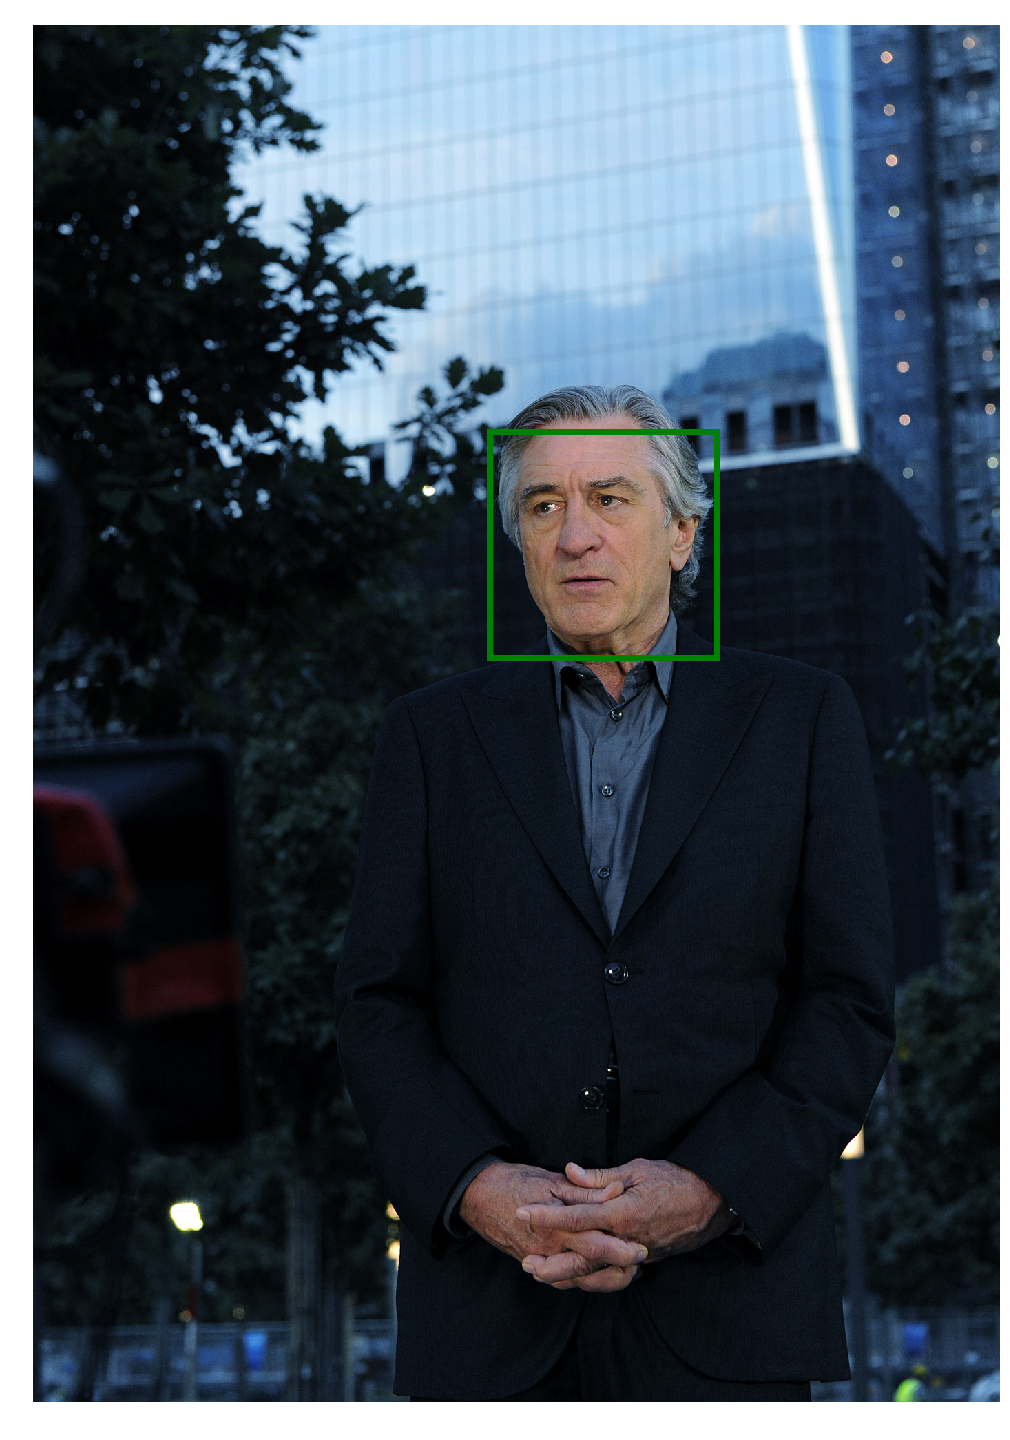
\includegraphics[width=\linewidth]{img/deniro_plt}
     \end{minipage}
\end{figure}

\begin{figure}[ht]
     \caption{Exemplo de imagem do conjunto de dados contendo mais de um rosto com a classificação correta.}
     \label{tab:dois_deniro_correto}
          \begin{minipage}[c]{0.62\linewidth}
          \begin{small}
          \centering
          \begin{tabular}{p{3.3cm} p{5cm}}\toprule
			   \textbf{Meta-dado} & \textbf{Valor} \\ \midrule
               ID Celebridade & 16349 \\
               Nome & Robert De Niro \\
               Endereço da imagem & \footnotesize{imdb$/$34$/$nm0000134$\_$rm17663 60064$\_$1943-8-17$\_$2010.jpg} \\
               Pontuação da Face & $5.12527$ \\
               Pontuação da Segunda Face & $5.08887$ \\
               Localização da Face & $(914.886, 1426.31, $ $287.31, 798.734)$ \\
               Data de Nascimento  & $1943-08-17$\\
               Ano da Foto & 2010 \\
               Gênero & Masculino \\
               \bottomrule
          \end{tabular}
     \end{small}
     \end{minipage}
     \hfill
     \begin{minipage}[c]{0.35\linewidth}
          \centering
          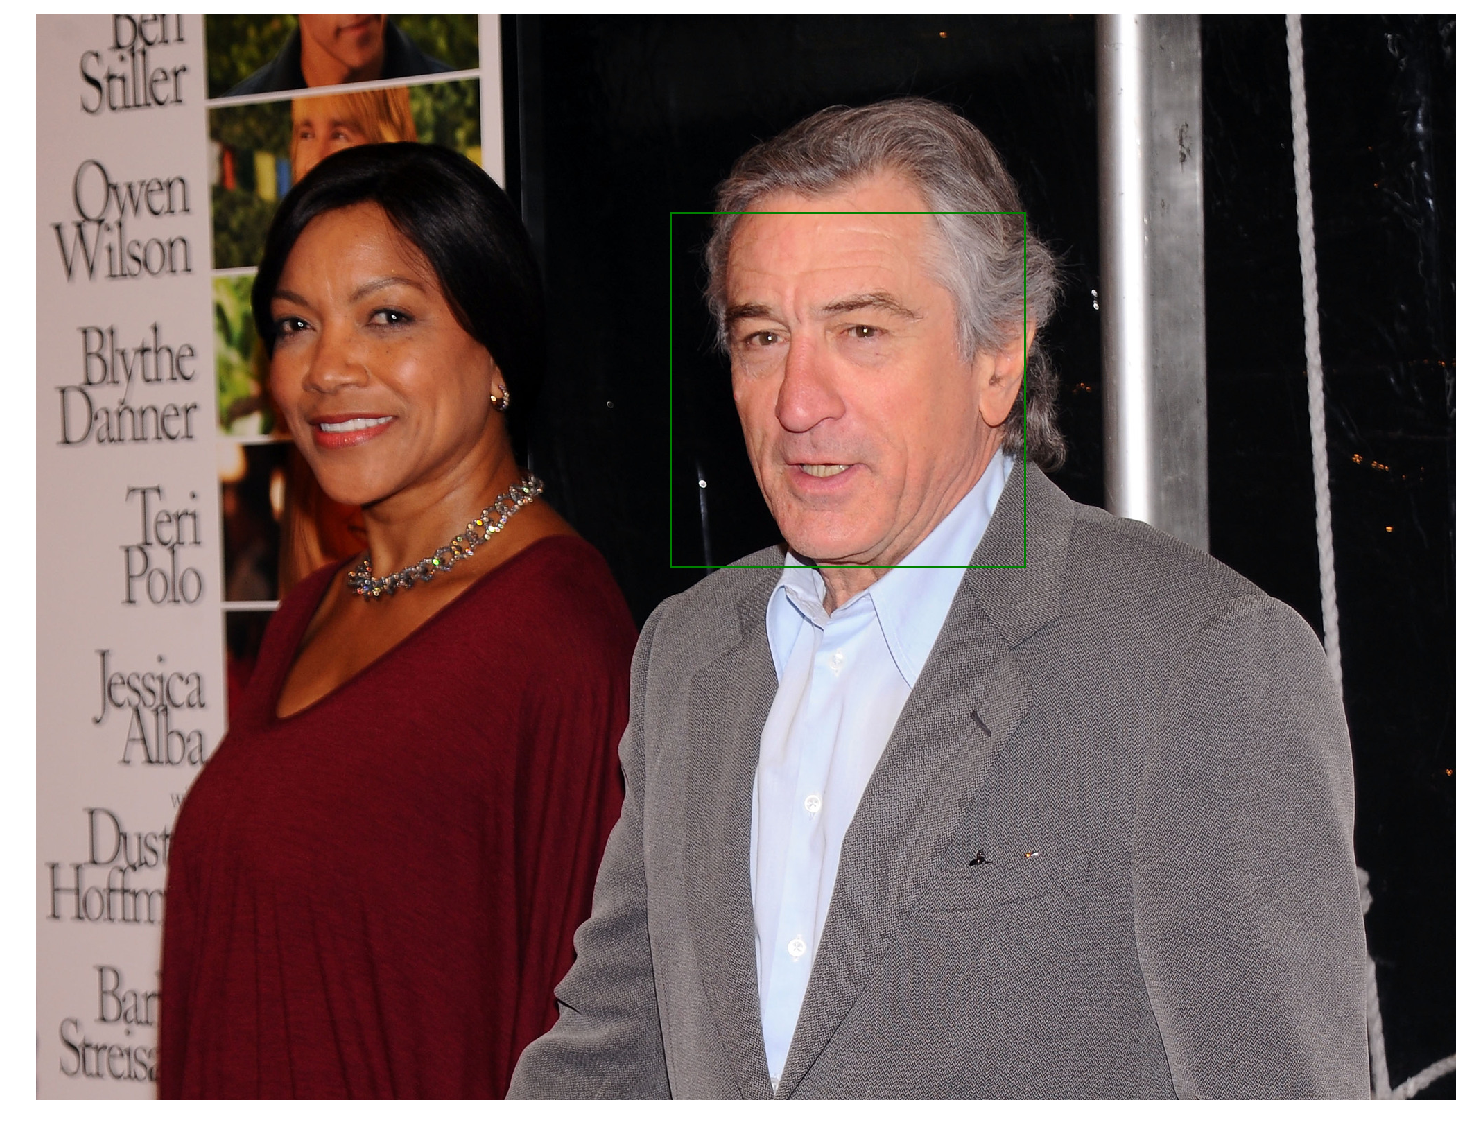
\includegraphics[width=\linewidth]{img/deniro_many_plt_correto}
     \end{minipage}
\end{figure}

\begin{figure}[ht]
     \caption{Exemplo de imagem do conjunto de dados contendo mais de um rosto com a classificação errônea.}
     \label{tab:dois_deniro_errado}
          \begin{minipage}[c]{0.62\linewidth}
          \begin{small}
          \centering
          \begin{tabular}{p{3.3cm} p{5cm}}\toprule
               \textbf{Meta-dado} & \textbf{Valor} \\ \midrule
               ID Celebridade & 16349 \\
               Nome & Robert De Niro \\
               Endereço da imagem & \footnotesize{imdb$/$34$/$nm0000134$\_$rm14800 44288$\_$1943-8-17$\_$2012.jpg} \\
               Pontuação da Face & $5.51656$ \\
               Pontuação da Segunda Face & $4.55379$ \\
               Localização da Face & $(1392.72, 1614.18, $ $225.55, 447.003)$ \\
               Data de Nascimento  & $1943-08-17$\\
               Ano da Foto & 2012 \\
               Gênero & Masculino \\ \bottomrule
          \end{tabular}
     \end{small}
     \end{minipage}
     \hfill
     \begin{minipage}[c]{0.35\linewidth}
          \centering
          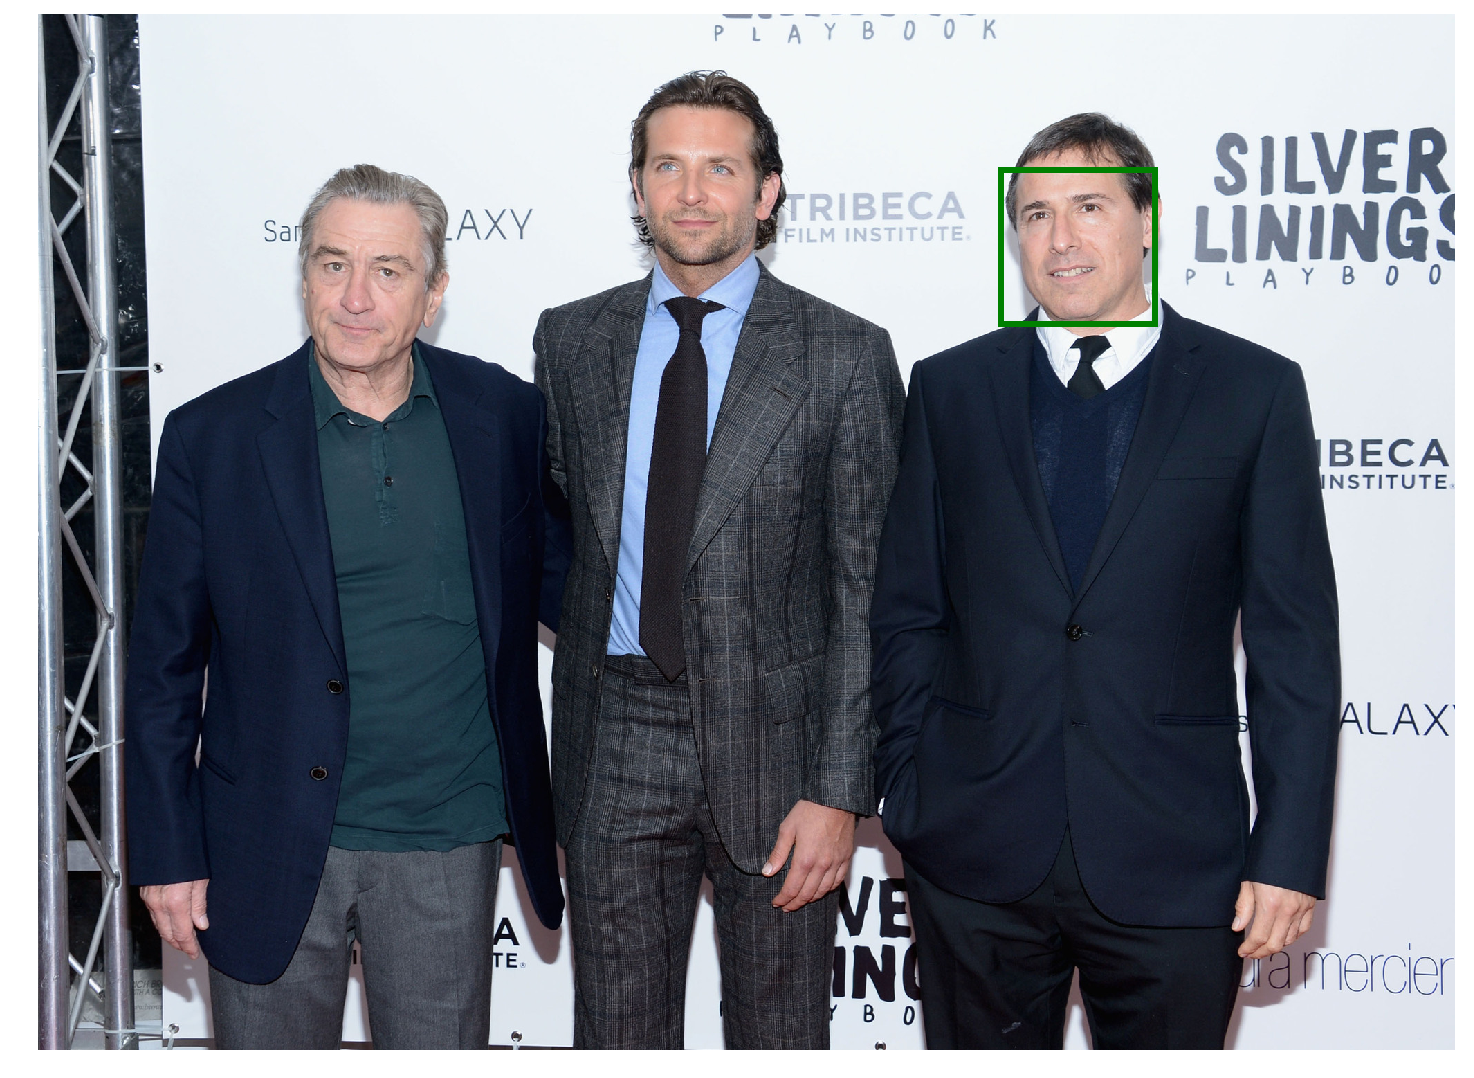
\includegraphics[width=\linewidth]{img/deniro_many_plt_errado}
     \end{minipage}
\end{figure}

A versão original das imagens do conjunto de dados IMDb ocupava 267 GB em disco. Porém, uma versão pré-processada dessas imagens está disponível, contendo as faces recortadas com $40\%$ da largura e altura da imagem original, totalizando $7,1$ GB de dados. Esta versão foi considerada neste trabalho.


\subsection{Limpeza e Pré-processamento dos dados}\label{subsec:limpeza}

A fim de adequar melhor o conjunto de dados para os modelos de CNNs utilizados, realizou-se uma limpeza e pré-processamento dos meta-dados e das imagens da base IMDb, que se iniciou com o cálculo do atributo alvo, a idade, a partir dos atributos originais fornecidos. A idade foi aferida através da data de nascimento da celebridade e do ano em que a fotografia em questão foi capturada.

Uma análise do conjunto de dados revelou a presença de itens com idade e gênero apresentando valores nulos, inválidos ou negativos, que foram descartados. Observou-se também a presença de múltiplos exemplos referentes à mesma pessoa com a mesma idade. Houve a remoção de tais exemplos, a fim de evitar que a apresentação de um mesmo rosto com a mesma idade provocasse \emph{overfitting} nos modelos. Exemplos atípicos, possivelmente resultados de rotulação incorreta, como idade maior que $100$ anos ou não compatível com os dados da celebridade referida nos meta-dados também foram descartados. Os atributos de pontuação de rostos foram úteis para identificar e remover exemplos em que não havia nenhum rosto identificado, ou em que havia mais de uma face na imagem. Este descarte foi realizado com o objetivo de eliminar rotulações errôneas, como a mostrada na Tabela \ref{tab:dois_deniro_errado}.

A última etapa consistiu na padronização das dimensões das imagens. Considerando a literatura, definiu-se o tamanho para $224 \times 224$ \emph{pixels} e o modo RGB como padrões. Por fim, após a padronização das imagens de entrada, o cálculo do atributo alvo idade, a adequação do caminho para as imagens em disco e a remoção de exemplos impróprios, seguiu-se o descarte dos outros meta-dados irrelevantes para a tarefa de estimação de idade de um indivíduo a partir de imagem. A data em que a foto foi tirada, nome, número de identificação, gênero, data de nascimento, localização do rosto da celebridade e pontuações de rostos nas imagens foram removidos.

Por fim, o conjunto de dados consolidado consiste de $47.950$ exemplos contendo imagens e idades de $14.607$ celebridades distintas, ocupando $1,2 GB$. O histograma de frequência da distribuição de idades de 0 a 100 anos presente nos exemplos da base de dados pode ser visualizado na Figura \ref{fig:hist}. Este total foi então dividido como proposto: conjunto de treinamento, contendo $70\%$ dos exemplos, ou seja, $33.565$ amostras; conjunto de validação, referente a $10\%$ dos dados, ou seja, $4.795$ itens; e, por fim, conjunto de testes, contendo os $20\%$ restantes, ou seja, $9.590$ exemplos.

\begin{figure}
    \centering
     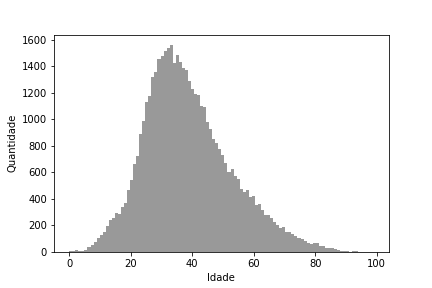
\includegraphics[width=0.7\textwidth]{img/idade_hist_clean}
     \caption{Histograma de frequência da idade do conjunto de dados utilizado.}
     \label{fig:hist}
\end{figure}

\subsection{Modelos de CNN Considerados} \label{subsec:modelos}
<<<<<<< HEAD
Levando em conta a adoção de CNNs como o modelo de ML a ser usado neste trabalho, considerou-se a utilização das arquiteturas LeNet e AlexNet. A implementação da AlexNet seguiu a prática atual de utilizar apenas uma GPU em seu treinamento, então as camadas dividas no trabalho original foram unificadas \cite{tensorflow:alexnet}. Todas as funções de ativação tangente hiperbólica disponíveis nas versões originais destas redes foram substituídas pela função \emph{ReLU}, por ser mais eficiente computacionalmente, evitar que o gradiente descendente tenda a zero e por promover uma convergência mais rápida \cite{maas2013rectifier}. Adotou-se um \emph{batch size} igual a $64$ para o treinamento, e o método de otimização do gradiente descendente foi o \emph{Adam}. O número de épocas e a taxa de aprendizado foram obtidas de maneira experimental, observando a perda obtida ao final de cada época.
=======
Levando em conta a adoção de CNNs como o modelo de Aprendizado de Máquina a ser usado neste trabalho, considerou-se a utilização das arquiteturas LeNet e AlexNet. A implementação da AlexNet seguiu a prática atual de utilizar apenas uma GPU em seu treinamento, então as camadas dividas no trabalho original foram unificadas \cite{tensorflow:alexnet}. Todas as funções de ativação tangente hiperbólica disponíveis nas versões originais destas redes foram substituídas pela função \emph{ReLU}, por ser mais eficiente computacionalmente, evitar que o gradiente descendente tenda a zero e por promover uma convergência mais rápida \cite{maas2013rectifier}. Adotou-se um \emph{batch size} igual a $64$ para o treinamento, e o método de otimização do gradiente descendente foi o \emph{Adam}. O número de épocas e a taxa de aprendizado foram obtidas de maneira experimental, observando a perda obtida ao final de cada época.
>>>>>>> master

A fim de caracterizar a tarefa de regressão proposta, as camadas de saída da LeNet e AlexNet com múltiplos neurônios voltados à classificação foram substituídas por apenas um neurônio com função de ativação \emph{ReLU}. Após análise dos resultados preliminares obtidos para estes modelos iniciais, substituiu-se a \emph{ReLU} da camada de saída por uma de suas variantes, chamada \emph{Leaky ReLU}, e expressa na Figura \ref{fig:lrelu}. A taxa de aprendizado inicial foi padronizada em um valor de $10^{-3}$ com decaimento de $10^{-10}$ para ambas as redes.

\begin{figure}[h!]
     \centering
     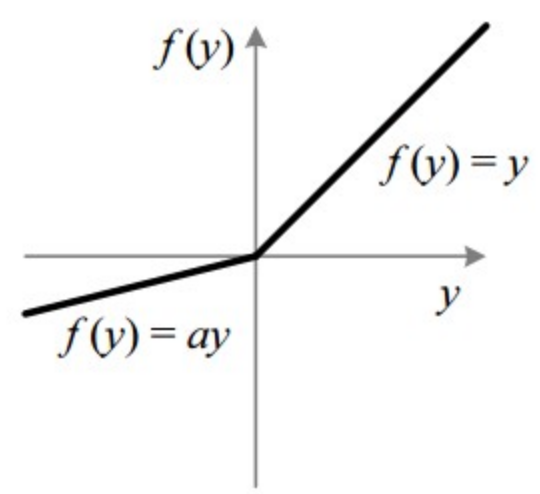
\includegraphics[width=0.3\textwidth]{img/lrelu}
     \caption{Função de Ativação \emph{Leaky ReLU}}
     \label{fig:lrelu}
\end{figure}

Na seção a seguir estão os resultados preliminares obtidos do treino dos modelos, hiperparâmetros e estratégias supracitados.
